\section{硬件优化}
\label{sec:hardware-optimization}

为 LLM 推理设计高效硬件具有挑战性，核心原因在于算术强度\footnote{算术强度是“计算量/访存量”比值，见 Roofline 模型（Sec.~\ref{sec:Rooflinemodel}）。}在不同阶段与负载配置下差异巨大。

prefill 阶段通常以 GEMM 批量处理 token，算术强度较高；
decode 阶段按 token 逐步生成，常落到 GEMV 或瘦 GEMM，算术强度较低。
此外，batch size 与 sequence length 的变化也会显著改变算术强度：
大 batch 往往提高算术强度，而长序列会增加 KV cache 读取访存压力。
这种“阶段+配置双重变化”使硬件设计必须考虑多场景最优。

因此本节围绕“如何应对算术强度变化”回顾硬件优化路径。

\subsection{空间架构（Spatial Architecture）}

LLM 的 decode 自回归特性意味着在大量应用中，时延主要耗在 decode。
其低算术强度本质来自对权重与 KV cache 的高频访存。

空间架构提供一种改进思路：
与传统“计算单元与主存反复交互”的时分复用方式不同，空间架构将计算分布到多个 PE 并行执行，让中间数据在 PE 间流动，减少回写 DRAM 的频次。

\begin{figure}[t]
    \centering
    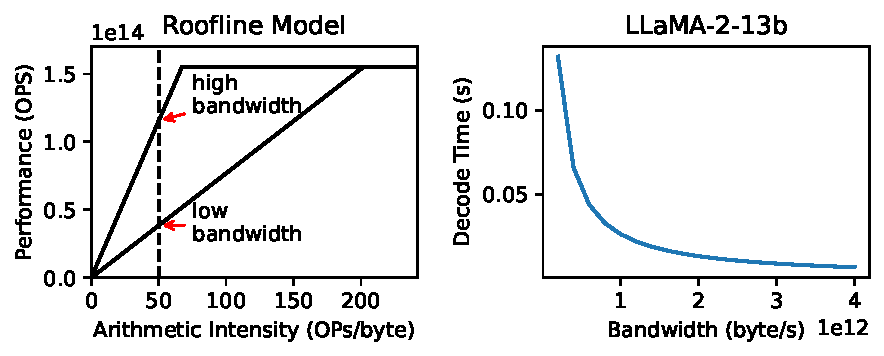
\includegraphics[width=0.95\linewidth]{ims/hardware_bandwidth.pdf}
    \caption{带宽变化对 Roofline 与 Llama-2-13b（batch=1, seq=1024）性能的影响。}
    \label{fig:hardware_bandwidth}
\end{figure}

在空间架构下，每个 PE 负责局部计算并与邻近 PE 通信，同时具备独立访存通路。
多 PE 并发访问提升系统总带宽，进而提升推理性能。
图~\ref{fig:hardware_bandwidth} 显示：总带宽提升时，decode 阶段线性层性能可显著增长。

实践方面，Groq 的 LPU~\citep{abts2022groq_lpu} 构建了面向 LLM 的空间系统，据报告在 Llama-2-70b 上可达每用户 300+ token/s~\citep{groq2023lpu_report}。
Graphcore IPU 也是可高效执行 LLM 的空间架构代表~\citep{graphcore_gradient_huggingface}。

\subsection{存内计算（Processing in Memory）}

LLM decode 常受“Memory Wall”限制。
该问题在体系结构领域长期存在，近年来 PIM（存内/近内计算）成为重要方向：将计算单元放入内存芯片内部，利用更高内部带宽并减少数据搬运。

近年来 DRAM-PIM 开始商用，有望缓解推理带宽瓶颈。
表~\ref{tab:pim-compare} 中，UPMEM PIM-DIMM~\cite{upmem} 是早期商用品，采用 DDR4-DIMM 内嵌 RISC 核，但并非面向深度学习设计，峰值带宽与吞吐难满足 LLM。
相比之下，Samsung HBM-PIM 将 MAC 集成到 HBM，内部带宽约 2TB/s，且算力约 1.2TFLOPS，更适合 1--2 Ops/Byte 区间算子。

\cite{choi2023unleashing} 提出用 HBM-PIM 加速 batched LLM 中低算术强度 KV-cache 处理，报告 GPU+HBM-PIM 系统可达 3.24$\times$ 提速。

SK-hynix 也提出基于 GDDR6 的 AiM~\cite{gddr-pim}，采用 BF16 MAC，单芯片约 1TFLOPS 与 1TB/s。
尽管尚未报告 LLM 数据，在 LSTM 任务上对比 GPU+HBM2 可达最高 10$\times$ 提升。

尽管 DRAM-PIM 对 memory-intensive 算子潜力显著，仍存在若干限制：
\begin{itemize}
\item \textbf{计算能力受限。}DRAM 工艺下晶体管速度与逻辑密度劣于同代 CMOS~\cite{devaux2019true}，且金属层少、布线密度低，难集成强算力单元。故更适于小 batch 或 KV 处理，大 batch 高计算场景仍需强主机。
\item \textbf{容量受限。}PIM 需占用部分存储区域构建计算单元，容量通常较标准内存减少约 50\%~\cite{hbm-pim}。对需承载大权重与 KV 的 LLM 场景是明显约束。
\item \textbf{PIM 间通信不足。}PIM 单元分布在各 DRAM bank 附近，跨单元聚合与同步不可避免；但现有 DRAM-PIM 互连能力有限~\cite{zhou2023dimm,jonatan2024scalability}，常依赖 CPU/GPU 中转，易形成系统低效。
\end{itemize}

\begin{table}[t]
\centering
\caption{Comparison of Commodity DRAM NMC Products}
\label{tab:pim-compare}
\resizebox{0.475\textwidth}{!}{
\begin{tabular}{|c|c|c|c|}
\hline
Product         &  PIM-DIMM & HBM-PIM          & AiM            \\ \hline
Technique  &       DDR4         & HBM2   & GDDR6  \\ \hline
PIM Units &  RISC Cores   & FP16 MAC   &  BF16 MAC      \\ \hline
Peak Bandwidth  &   80.4 GB/s    per DIMM          & 2 TB/s per cube   & 1 TB/s per chip  \\ \hline
Peak Throughput &   43.8 GOP/s per DIMM             & 1.2 TFLOPS & 1 TFLOPS \\ \hline
%  Arithmetic Intensity        &         0.54 OP/Byte       & 0.6 OP/Byte           & 1 OP/Byte          \\ \hline
\end{tabular}
}
\end{table}

\subsection{新数据格式}
\label{sec:dataformat}

神经网络训练通常使用 16/32bit 高精度浮点。
高精度 FP 同时兼顾表示精度与范围，但硬件实现复杂，不利于高效推理。

为降低硬件开销，均匀量化将高精度 FP 映射为低精度整数，替代昂贵浮点逻辑。
但均匀量化难同时兼顾“范围与精度”，且常需额外算法设计与校准开销来保精度。

非均匀量化尝试通过非均匀分桶与比特分配提升低比特表示精度，但在通用 CPU/GPU 上部署难度更高~\citep{gholami2022survey}。
总体上，现有格式难同时满足：高精度、宽范围、高效率、低调参成本。
因此大量工作在探索更适配 LLM 的数据格式。

\begin{table}[htbp!]
\centering
\resizebox{\linewidth}{!}{%
\begin{tabular}{cccc}
    \hline
    \textbf{维度} & \begin{tabular}{@{}c@{}} \textbf{浮点} \\ \textbf{格式} \end{tabular} & \begin{tabular}{@{}c@{}} \textbf{均匀} \\ \textbf{量化} \end{tabular} & \begin{tabular}{@{}c@{}} \textbf{非均匀} \\ \textbf{量化} \end{tabular} \\
    \hline
    精度        & Good & Bad & Medium \\
    范围        & Good & Bad & Medium  \\
    硬件效率    & Bad  & Good & Bad  \\
    转换成本    & Good  & Bad & Medium  \\
    \hline
\end{tabular}
}
\caption{浮点、均匀量化与非均匀量化对比}
\label{tab:data_format_comparison}
\end{table}

工业界路径之一是从高精度 FP 逐步降低 exponent/mantissa 比特。
近期研究~\citep{micikevicius2022fp8,sun2019hybrid} 表明多类模型（含 LLM）可从 FP16 直接迁移到 FP8 而精度损失有限。
低比特浮点因“高效率+低改造成本”受到硬件厂商重视：
NVIDIA 在 H100 中集成 FP8 Tensor Core~\citep{nvidiahopperarchitecture}，Tesla Dojo 引入可配置 CFloat8~\citep{tesladojotechnology}。

学术界也在推进低比特浮点用于 LLM：
ZeroQuant-FP~\citep{wu2023zeroquant} 探索 FP4/FP8；
ZeroQuant-(4+2)~\citep{wu2023zeroquant1} 与 FP6-LLM~\citep{xia2024fp6} 探索 FP6 权重量化；
LLM-FP4~\citep{liu2023llm} 将权重与激活均压到 FP4。
这些工作证明了更低比特浮点在准确性与效率上的可行性。

另一类研究改进编码方式本身：
可变长度编码允许在单值内部动态分配子字段比特，提升“范围-精度”折中能力。
代表工作有 ALPS~\citep{langroudi2021alps}、ANT~\citep{guo2022ant}、Dybit~\citep{zhou2023dybit}。

还有跨值协同编码方向：
离群值感知量化（OLAccel~\citep{park2018energy}、GOBO~\citep{zadeh2020gobo}、OliVe~\citep{guo2023olive}）对关键大幅值单独处理；
bit-sharing（AdaptivFloat~\citep{tambe2020algorithm}、MX~\citep{darvish2023shared}）在块级共享信息，兼顾精度与效率。

\begin{table}[htbp!]
\centering
\resizebox{\linewidth}{!}{%
\begin{tabular}{ccc}
    \hline
    \textbf{方法} & \textbf{描述} & \textbf{收益} \\
    \hline
    低比特浮点 & 减少指数与尾数比特 & Efficiency $\uparrow$ \\
    可变长度编码 & 动态调整子字段位宽 & Precision $\uparrow$ \\
    离群值感知量化 & 对离群值定制编码 & Precision $\uparrow$ \\
    Bit-sharing 编码 & 块内共享公共信息 & Precision $\uparrow$ \\
    \hline
\end{tabular}
}
\caption{新数据格式改进方向总结（通常以较小副作用换取收益）}
\end{table}

\subsection{新型处理单元（PE）}

除访存瓶颈外，业界也在探索专用处理单元以增强 LLM 关键算子计算效率。
这些单元针对 Transformer 负载定制，较通用 CUDA core 等可提供更高性能密度。

NVIDIA 在 H100 中引入 Transformer Engine，可按层统计动态选择 FP16/FP8 执行精度，在精度可控前提下提升性能。
也有工作针对注意力机制设计专用加速器~\citep{kao2023flat,qin2023fact}。
此外，FPGA 路径（如 DFX~\citep{hong2022dfx}、FlightLLM~\citep{zeng2024flightllm}）也在持续探索 LLM 推理加速。
